%!TEX root = ../projecto.tex
\section{Related Work} % (fold)
\label{sec:related_work}
In this section we will start by generally describing what Clustering is and how it works at subsection \ref{sub:clustering}, then at subsection \ref{sub:self_organizing_maps} it will be outlined how Self-organizing \cite{Kohonen1990}maps function, which is the Document Clustering algorithm used on this project.


\subsection{Document Clustering} % (fold)
\label{sub:clustering}
Document clustering is an optimal division of data into cathegories without prior knowledge of the data that is being organized, based only on the similarity between documents. Due to the fact that no prior knowledge of the date has to be known Document Clustering is labeled as Unsupervised Machine Learning.

Yuan-Chao Liu et Al \cite{Liu2012b} described that Document Clustering can be used to a variety of Computer Science fields, such as:
\begin{itemize}
  \item Natural Language Preprocessing.
  \item Automatic Sumarization.
  \item User preference mining.
  \item Improve Text classification results.
\end{itemize}

In regard to document categorization there are two main types of Document Clustering, Hard Clustering and Soft Clustering. In Hard Clustering one document can only belong to one cluster, while in Soft Clustering one document can belong to multiple clusters. 

In regard to document categorization \citet{Springorum1998} performed hard and soft clustering with SOMs \citep{Kohonen1990} while identifying polysemous German Propositions. They used regular SOMs to create multiple hard clusters and used Centroid-Based or Preposition-based softening to create Soft Clusters from the Hard Clusters.

The general mathematical description of Document Clustering can be seen in \ref{fig:1_Text_Clustering_Main_Framwork}
\begin{figure}
  \begin{center}
    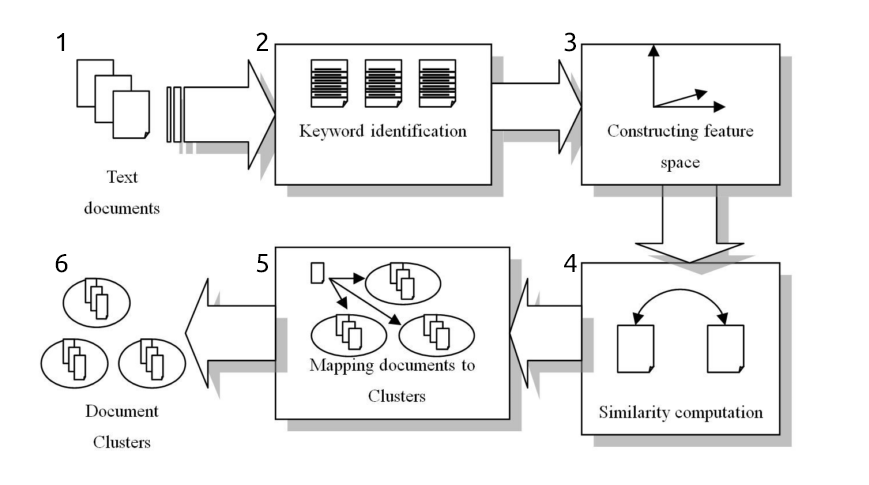
\includegraphics[width=12cm]{images/1_Text_Clustering_Main_Framwork.png}
  \end{center}
  \caption{ Text Clustering Main Framework from \citet{Dozono2012} }
  \label{fig:1_Text_Clustering_Main_Framwork}
\end{figure}
In the first step a data set must be provided in order to cluster the documents. 
The second step "Keyword identification" is where non relevant words are removed from the documents. \citet{Kang2003} proves that keyword removal improves clustering. Another way to extract features is to differentiate text features by analizing the document corpora. For example if the dataset is composed from HTML or XML documents it is possible to identify more relevante features due to the characteristics of the markup. In \ref{sub:topic_detection_on_twitter} it will be described twitts characteristics as a document and in \ref{sec:architecture} how feature extraction will be implemented on this project.
"Constructing the Feature Space" is characterized by converting the keywords of each document into vectors, the most common algorithm used for this task is SVM (Support Vector Machines). In SVM each vector dimension means one detected key word and each document is represented by the vector of keywords in the feature space. This process and keyword removal is described in Figure \ref{fig:2_svm}.
Due to the way documents are represented in SVM it is normal that vectors become very large and full of zeros ( keywords not present) and it is needed to use sparse vectors to represent the documents in a more efficient way.

\begin{figure}
  \begin{center}
    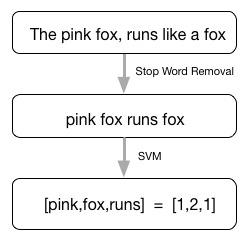
\includegraphics[width=5cm]{images/2_svm.jpg}
  \end{center}
  \caption{ Stop word removal and transformation to Vector Space Model }
  \label{fig:2_svm}
\end{figure}

Dimensional reduction is done after the construction of the vector space model, in order to reduce the size of the vector space. There are two main ways to do this PCA (Principal Component Analysis) and LSI (Latent Semantic Indexing). PCA calculates the k eigenvectors of the co-variance of the document matrix, which reduces the size of the matrix to k. LSI (Latent Semantic Indexing) works just like PCA but the eigenvectors are calculated directly from the document matrix.

There are two main strategies for Document Clustering, Complete strategie where the data set does not change and Incremental where initial number of document can increase by adding new documents. After a new document is added it can be merged into a existing cluster, or can be separated as a new category. While adding new documents it might be needed to re run the clustering algorithm. 

After the algorithm converges, cluster similarity can be calculated in multiple ways:
\begin{itemize}
  \item Shortest Distance Method: Shortest distance between two members of different clusters.
  \item Longest Distance Method: Longest distance between two members of different clusters.
  \item Group Average Method: The average distance between all elements of both clusters.
  \item Centric Method: The distance between the center of two clusters.
\end{itemize}

There many clustering algorithms, here we will focus on the three most popular.K-means works by randomly selecting k documents as the cluster centroids, then assign each document to the nearest centroid, and finally recalculate the the centroid with new added documents. The algorithm should be executed until convergence which reflects in the centroids stop changing. K-means has the advantage that the number of centroids must be selected before starting the algorithm.
AHC or Agglomerative Hierarchical Clustering is hierarquical clustering algorithm where clusters have sub-clusters which have subclusters. Like K-means it is also a simple algorithm that starts by calculating the similarity matrix, then each document is seen as a cluster and finally merge the nearest two clusters into one and update the similarity matrix. The algorithm ends when there is only one cluster or due to clustering entropy.An AHC classic example is species taxonomy where species have subspecies which have subspecies, etc.
Lastly there is Self-organizing Maps introduces by \citep{Kohonen1990} which will be used in the thesis and will be detailedly described in the next subsection \ref{sub:self_organizing_maps}.
% subsection clustering (end)


\subsection{Self-Organizing Maps} % (fold)
\label{sub:self_organizing_maps}
% subsection self_organizing_maps (end)


\subsection{Topic Detection on Twitter} % (fold)
\label{sub:topic_detection_on_twitter}
% subsection topic_detection_on_twitter (end)
% section related_work (end)


\begin{itemize}
  \item What did we know about the problem before I did this study? 
  \item What did we do different from previous works? 
  \item Discuss the relevant primary research literature 
  \item Works should be organized by their relevant characteristics 
  \item Comment on why it is relevant for your work 
  \item Comment on what your work does differentely 
\end{itemize}